\section{\framework: Design Overview}
\label{sec:design-overview}

\begin{figure*}[t]
    \centering
    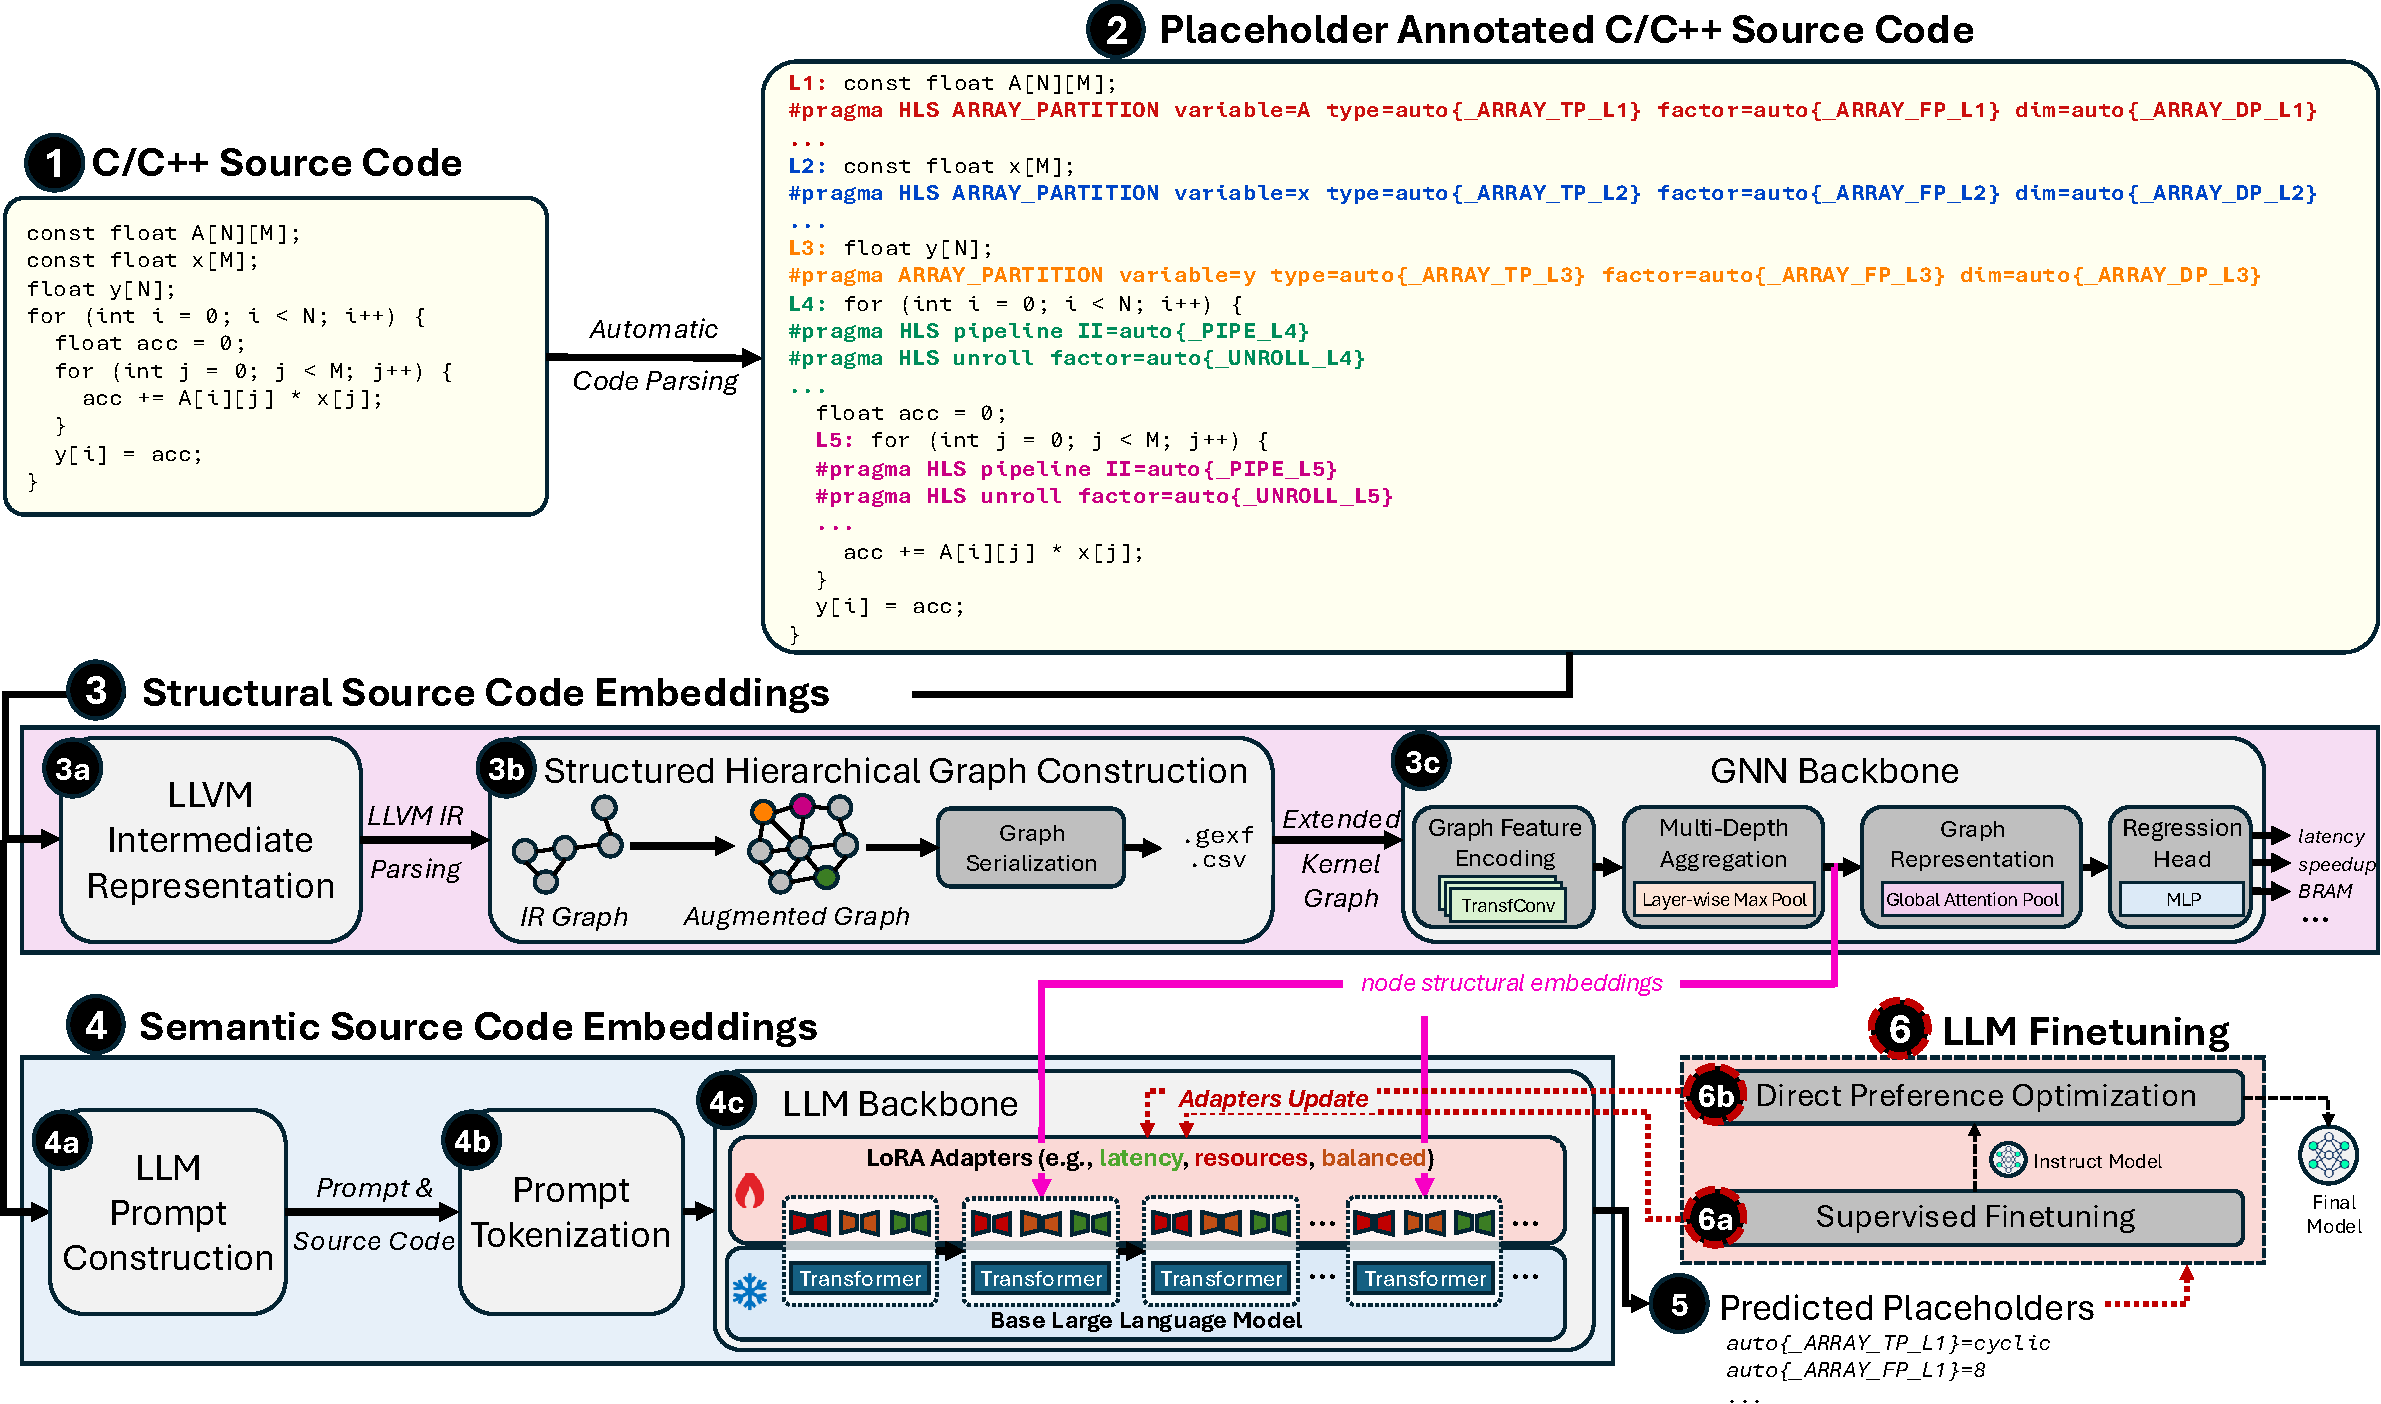
\includegraphics[width=\textwidth]{figures/02__Methodology/Proposed-Architecture-crop.pdf}
    \caption{\framework design overview. Given a C/C++ kernel and target request, \framework identifies directive action points, encodes semantic and compiler-derived structural representations, fuses them through gated cross-attention, and predicts objective-aware pragma values. Cold components denote frozen modules, while hot components denote trainable parts. \EV{should be updated after the figure update}}
    \label{fig:design-overview}
\end{figure*}

\figuretodo{Edit the existing architecture figure :
(1) labeled C/C++ + kernel\_info.txt -> cgeist/Polygeist ->
Affine / SCF / MemRef / Arith / Func MLIR -> deterministic action-aligned graph;
(2) GNN QoR heads as training supervision only, with pre-head action-point embeddings exported to absolute L\_k memory slots;
(3) Stage 1 as target-aware SFT with no structural input;
(4) Stage 2 as frozen Stage 1 plus post-self-attention gated cross-attention at layers 8/16/24/32, with compiler-relational routing and value-only application;
(5) Stage 3 DPO; (6) a small AUTO branch: selector -> supported clock -> ordinary specified-clock SALT-HLS policy.
The prompt box must contain objective, FPGA, BRAM/DSP/FF/LUT budgets, and clock.
Preserve the existing circled workflow and hot/cold visual language.}

% To address the limitations in \S\ref{sec:motivation} \EV{maybe we should close motivation with the overall limitations to have this link for starting to describe our framework}, we propose \framework, a target-conditioned hybrid framework for direct HLS pragma optimization. Training is Pareto-driven in the sense that supervision is constructed from objective-ranked feasible designs within a fixed kernel/device/clock/budget context; inference itself is not a Pareto search. The design follows three principles:

% \begin{enumerate}[leftmargin=*,label=\textbf{(\arabic*)},labelsep=0.3em,topsep=2pt,itemsep=2pt]
%     \item \textbf{Joint structural \& semantic modeling.} \framework combines compiler-derived graph representations with language-model reasoning to capture both program organization and source-level semantics. The GNN encodes explicit relations among loops, regions, values, and memory operations; the LLM interprets source context and the requested optimization target. Gated cross-attention connects the two views at directive decisions. \EV{slightly repetitve?}

%     \item \textbf{Directive-level decision abstraction.} Instead of generating arbitrary HLS code, \framework predicts values for source-derived directive placeholders placed at eligible loop and array action points. The action contract \EV{change action contract} fixes \emph{where} a supported pragma may act and provides a set of accepted directive values including a no-op value which allows the policy to decide whether the action is activated. This substantially reduces syntax/placement errors without implying that every generated configuration is synthesizable or resource-feasible.

%     \item \textbf{Objective- and target-aware optimization.} The policy conditions on one of three objectives---latency, area, or latency-area product (ADP)---and on the target context: target device, available BRAM/DSP/FF/LUT budget, and clock period. The exact objective metric and target protocol are defined in \S\ref{subsec:eval-objectives}. \EV{wwhat are the objective metric and the target protocol?}
% \end{enumerate}

% Figure~\ref{fig:design-overview} presents the end-to-end workflow. Given an input C/C++ kernel (\circled{1}), the framework identifies candidate optimization action points---loops and arrays---and augments them with parameterized directive placeholders (\circled{2}). Each action identity $L_k$ is shared across the source prompt, the compiler graph, and the structural memory, providing a deterministic alignment between the language and graph representations.

% For the \textit{structural representation} (\circled{3}), the source is lowered with cgeist/Polygeist to structured MLIR~\cite{lattner2021mlir}. An edge-aware GNN is trained with QoR supervision \EV{with what loss does the GNN gets trained, with what goal} and exports deterministic action-point embeddings before its prediction heads. \EV{repetition} For the \textit{semantic/target representation} (\circled{4}), a decoder-only code LLM processes the source together with objective, target device, available resource component-wise budget, and clock. Stage~1 learns directive values without structural input; Stage~2 freezes Stage~1 and trains only gated cross-attention at layers 8/16/24/32 using compiler-relational action routing \EV{why at those layers and why compiler-relational routing}. The detailed graph creation and memory extraction are given in \S\ref{sec:detailed-design}.

% Finally, \framework emits one complete directive assignment (\circled{5}). Stage~3, preference-aligns same-context complete design actions without changing the target interface. AUTO-clock adaptation is evaluated as a separate clock-selection component; after selecting a supported period, directive generation uses the unchanged specified-clock policy.

To address the limitations identified in
\S\ref{sec:motivation}, \framework learns a direct mapping from a
source program and deployment request to one complete HLS directive
configuration. Training is Pareto-driven: supervision is selected from
measured designs that are feasible under the same
kernel/device/clock/resource context, whereas deployment performs no
Pareto search.

Figure~\ref{fig:design-overview} summarizes the workflow. A deterministic
source analyzer first identifies the loop and array locations at which
supported HLS decisions may be made and assigns each location a stable
action identity $L_k$ (\circled{1}--\circled{2}). Each action exposes a
finite source-derived value domain, including a no-op choice. The same
action identity is subsequently used by the language representation and
the compiler representation, providing the correspondence required for
structural fusion.

The two model paths are trained separately before they are connected.
On the language path, Stage~1 fine-tunes a decoder-only code model to
predict directive values from the source and target request alone. The
request is
%
\[
\tau=(d,c,\mathbf b),\qquad
\mathbf b=(b_{\rm BRAM},b_{\rm DSP},b_{\rm FF},b_{\rm LUT}),
\]
%
together with the optimization objective. Latency minimizes synthesized
cycles; area minimizes the mean normalized BRAM/DSP/FF/LUT utilization;
and ADP minimizes their latency--area product among designs feasible
under $\tau$ (formal definitions in \S\ref{subsec:eval-objectives}).

In parallel, the structural path raises the pragma-free C/C++ kernel
through cgeist/Polygeist to structured MLIR and converts the resulting
compiler representation into an action-aligned relational graph
(\circled{3}). A separately trained edge-aware GNN receives QoR
supervision from synthesized latency and resource measurements. Its
prediction heads provide training supervision only: the final policy
exports hidden action representations before those heads rather than
using predicted QoR to rank or rerank candidate designs.

Stage~2 freezes the Stage~1 policy and learns gated cross-attention from
directive-value positions to the corresponding structural memory.
Structural fusion is distributed across four decoder depths
(layers 8, 16, 24, and 32), providing repeated access to compiler evidence
while leaving most of the pretrained computation unchanged. Rather than
attending to every action indiscriminately, each directive decision is
restricted to its own structural slot and compiler-related action slots;
the exact relation construction is described in
\S\ref{subsubsec:graph-construction}. Stage~3 finally preference-aligns
complete configurations compared under the same target context.

For a specified-clock request, the resulting system emits one complete
configuration in a single policy invocation (\circled{5}); HLS is used
only afterward for validation and measurement. AUTO-clock operation is a
separate lightweight selector: it first chooses one supported period and
then invokes the unchanged specified-clock policy.

